\section{Introduction}%
\label{sec:introduction}

\begin{figure*}
    \centering
    \subfloat[\textmd{Technical comparison between generative SSL methods. }]{
        \adjustbox{valign=b}{
        \small
        \renewcommand\tabcolsep{3pt}
        \begin{tabular}{@{}lccccccc@{}}
\toprule[1.2pt]
Methods  & \makecell[c]{Feat.\\Loss}   & AE         & \makecell[c]{No\\Struc.}  & \makecell[c]{Mask\\Feat.} & \makecell[c]{GNN\\Decoder}    & \makecell[c]{Re-mask\\Dec.}   & Space              \\ \midrule
VGAE~\cite{kipf2016variational} & n/a      & \Checkmark & -          & -          & -             & -    & $\mathcal{O}(N^2)$ \\
% EP~\cite{garcia2017learning}       & MSE    & \Checkmark & \Checkmark & -          & -            & -    & $\mathcal{O}(N^2)$ \\
ARVGA~\cite{pan2018adversarially}    & n/a      & \Checkmark & -          & -          & -          & -    & $\mathcal{O}(N^2)$ \\
MGAE~\cite{wang2017mgae}     & MSE    & \Checkmark & -          & \Checkmark & -                    & -    & $\mathcal{O}(N)$ \\
GALA~\cite{park2019symmetric}     & MSE    & \Checkmark & \Checkmark & -          & \Checkmark      & -    & $\mathcal{O}(N)$  \\
GATE~\cite{amin2020gate}     & MSE    & \Checkmark & -          & -          & \Checkmark           & -    & $\mathcal{O}(N)$   \\
AttrMask~\cite{hu2020strategies} & CE     & \Checkmark & \Checkmark & \Checkmark & -                & -    & $\mathcal{O}(N)$   \\
GPT-GNN~\cite{hu2020gpt}  & MSE    & -          & -          & \Checkmark & -                       & -    & $\mathcal{O}(N)$   \\
AGE~\cite{cui2020adaptive}     & n/a      & \Checkmark & -          & -          & -                & -    & $\mathcal{O}(N^2)$  \\
NodeProp~\cite{jin2020self} & MSE    & \Checkmark & \Checkmark & \Checkmark & -                     & -    & $\mathcal{O}(N)$ \\
% RASSL~\cite{zhu2020self}    & MSE    & \Checkmark & -          & -          & -           & $\mathcal{O}(N^2)$   \\ 
\midrule
% \model   & Cosine & \Checkmark & \Checkmark & \Checkmark & \Checkmark  & $\mathcal{O}(N)$ \\ \bottomrule[1.2pt]
\model   & SCE & \Checkmark & \Checkmark & \Checkmark & \Checkmark  & \Checkmark & $\mathcal{O}(N)$ \\ \bottomrule[1.2pt]
\end{tabular}

        \label{fig:cmp_tab}}}
    \ 
    \
    \subfloat[\textmd{The effect of \model designs on the performance on Cora dataset. %\model significantly improves the accuracy with starred operations.
    }]{           
        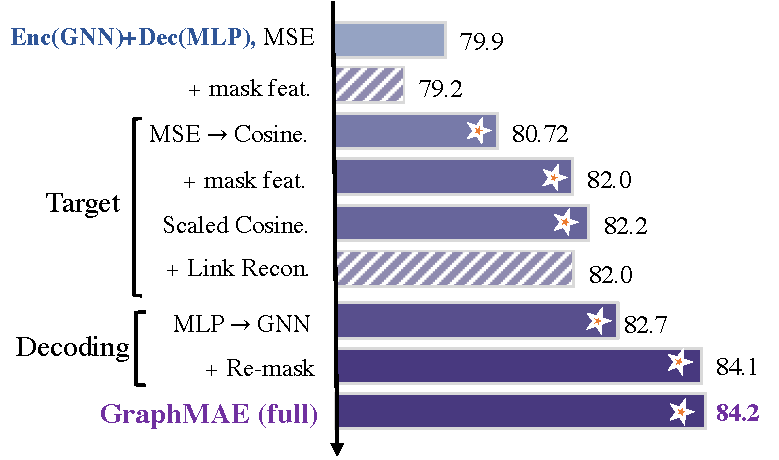
\includegraphics[width=0.48\linewidth,valign=b]{imgs/GraphMAEXT.pdf} 
        \label{fig:design_eff}          
        }
    \caption{Comparison between generative SSL methods and the effect of \model design. \textmd{
    %(a). The comparison between generative SSL methods. 
    %(b). The effect of \model design choices on .
    \textit{AE}: autoencoder methods;
    \textit{No Struct.}: no structure reconstruction objective;
    \textit{Mask Feat.}: use masking to corrupt input features;
    \textit{GNN Decoder}: use GNN as the decoder;
    \textit{Re-mask Dec.}: re-mask encoder output before fed into decoder;
    \textit{Space}:  run-time memory consumption;
\textit{MSE}: Mean Squared Error; 
    \textit{SCE}: Scaled Cosine Error; 
    \textit{CE}: Cross-Entropy Error;
    \textit{SCE} represents our proposed Scaled Cosine Error.}
    }
    \label{fig:cmp_deg}
    % \vspace{-3mm}
\end{figure*}


Self-supervised learning (SSL), which can be generally categorized into generative and contrastive methods~\cite{liu2021self}, has found widespread adoption in computer vision (CV) and natural language processing (NLP). 
%and graph machine learning. 
While contrastive SSL methods have %\zfj{been blossoming, }
 experienced an emergence in the past two years, 
such as MoCo~\cite{he2020momentum}, generative SSL has been gaining steadily increasing significance thanks to several groundbreaking practices, such as the well-established BERT~\cite{devlin2019bert} and GPT~\cite{Radford2019LanguageMA} in NLP as well as the very recent MAE~\cite{he2021masked}  %iBOT~\cite{zhou2021ibot} 
in CV. 



However, in the context of graph learning, % albeit prior efforts on GAEs, 
contrastive SSL has been the dominant approach, especially for two important tasks---node and graph classifications~\cite{velivckovic2018deep, qiu2020gcc,hassani2020contrastive}. 
Its success has been largely built upon relatively complicated training strategies. 
For example, the bi-encoders with momentum updates and exponential moving average are usually indispensable to stabilize the training of GCC~\cite{qiu2020gcc} and BGRL~\cite{thakoor2021bootstrapped}. 
Additionally, negative samples are  necessary for most contrastive objectives, often requiring arduous labor to sample or construct from graphs, e.g., GRACE~\cite{zhu2020deep}, GCA~\cite{zhu2021graph}, and DGI~\cite{velivckovic2018deep}. 
Finally, its heavy reliance on high-quality %and label-invariant 
data augmentation proves to be the 
pain point  
%Achilles heel 
of contrastive SSL, e.g., CCA-SSG~\cite{zhang2021canonical}, as graph augmentation is mostly based on heuristics whose effectiveness varies drastically from graph to graph. 
%, and some of them can be unscalable at larger scales (e.g., diffusion in MVGRL~\cite{hassani2020contrastive}).

%data augmentation, negative sampling, bi-encoders and other techniques to stabilize training


Self-supervised graph autoencoders (GAEs) can naturally avoid the aforementioned issues in contrastive methods, as its learning objective is to directly reconstruct the input graph data~\cite{kipf2016variational,garcia2017learning}.   
%Generative SSL in graphs, including graph autoregressive model (GAR) and graph autoencoders (GAEs), has also been studied for long. 
%As a typical GAR model, 
Take VGAE for example, it~\cite{kipf2016variational} targets at predicting missing edges. 
EP~\cite{garcia2017learning} instead proposes to recover vertex features. 
GPT-GNN~\cite{hu2020gpt} proposes an autoregressive framework to perform node and edge reconstruction iteratively. 
Later GAEs, 
including ARVGA~\cite{pan2018adversarially}, MGAE~\cite{wang2017mgae}, GALA~\cite{park2019symmetric}, GATE~\cite{amin2020gate}, and AGE~\cite{cui2020adaptive},
majorly focus on the objectives of link prediction and graph clustering. 
%Compared to GAR's impractical assumption on graph generating orders, GAEs holds little assumption and thus find more widespread applications.


\vpara{Dilemmas.} 
Despite their simple forms and various recent attempts 
% on them ~\cite{you2020does,manessi2021graph,zhu2020self,jin2020self,hu2020strategies}, the development of self-supervised GAEs has been 
on them ~\cite{you2020does,jin2020self,hu2020strategies,park2019symmetric,amin2020gate,cui2020adaptive}, the development of self-supervised GAEs has been 
thus far lagged behind contrastive learning. 
%Despite a number of recent attempts~\cite{you2020does,manessi2021graph,zhu2020self,jin2020self,hu2020strategies} to handle such challenges with autoencoders, 
To date, there have been no GAEs succeeding to achieve a comprehensive outperformance over contrastive SSL methods, especially on node and graph classifications, which have been significantly advanced by neural encoders, 
% e.g., graph neural networks (GNNs); 
e.g., graph neural networks. 
%the progress of GAEs in graph has lagged behind NLP and CV. 
To bridge the gap, we  analyze %the deficiency of 
existing GAEs and identify the  issues that may negatively affect the progress of GAEs. 
Note that though previous GAEs may have individually tackled one or two of these issues below, 
%defects, 
none of them collectively deals with the four challenges. 
%We try to shed some lights on this gap by analyzing the following problems of existing GAEs:


%\begin{itemize}[leftmargin=*,itemsep=0pt,parsep=0.2em,topsep=0.3em,partopsep=0.3em]
%(i) 
%\item 
First, the structure information may be over-emphasized. 
Most  GAEs leverage  link reconstruction as the objective to encourage the topological closeness between neighbors~\cite{kipf2016variational,pan2018adversarially,wang2017mgae,amin2020gate,hu2020gpt,cui2020adaptive}. 
% \dong{reference all methods in fig 1a that fits here, also do this for the next three} 
Thus, prior GAEs are usually good at link prediction and node clustering, but unsatisfactory on node and graph classifications. 

%(ii) 
%\item 
Second, feature reconstruction without corruption may not be robust. 
For GAEs~\cite{kipf2016variational,pan2018adversarially,park2019symmetric,amin2020gate,cui2020adaptive} that leverage feature reconstruction, most of them still employ the vanilla architecture that risks learning trivial solutions. 
However, the denoising autoencoders~\cite{vincent2008extracting} that corrupt input and then attempt to recover it have been widely adopted in NLP~\cite{devlin2019bert}, which might be applicable to graphs as well.

%(iii) 
%\item 
Third, 
the mean square error (MSE) can be sensitive and unstable. 
To the best of our knowledge, 
all existing GAEs with feature reconstruction~\cite{wang2017mgae,park2019symmetric,amin2020gate,hu2020gpt,jin2020self} have adopted MSE as the criterion without additional precautions. 
However, MSE is known to suffer from varied feature vector norms and the curse of dimensionality~\cite{Friedman2004OnBV} 
% \dong{xx}, 
and thus can cause the collapse of training for autoencoders. 
%\todo{polish the reason}

%(iv) 
%\item 
Fourth, 
the decoder architectures are of little expressiveness. 
Most GAEs~\cite{kipf2016variational,pan2018adversarially,wang2017mgae,hu2020strategies,hu2020gpt,cui2020adaptive,jin2020self} leverage  MLP as their decoders. % by following BERT. 
However, the targets in language are one-hot vectors containing rich semantics, while in graphs, most of our targets are less informative feature vectors (except for some discrete attributes such as those in chemical graphs). 
In this case, this trivial decoder (MLP) may not be strong enough to bridge the gap between encoder representations and decoder targets for graph features.

%\end{itemize}

% Though previous GAEs may have individually tackled one or two of the above 
% issues, 
%defects, 
% none of them jointly deals with the four challenges as a whole. 
%The lack of a unified GAE solution to supersede contrastive self-supervised graph methods across extensive benchmarks.




\vpara{Contributions.}
In light of the above observations, the goal of this work is to examine to what extent we can 1) mitigate the issues faced by existing GAEs and 2) further enable GAEs to match or outperform contrastive graph learning techniques. 
To this end, we present a masked graph autoencoder \model for self-supervised graph representation learning. 
By identifying the critical components in GAEs, we add new designs and also improve existing strategies for \model, unleashing the power of autoencoders for graph learning. 
%\dong{to update this}
Figure \ref{fig:cmp_tab} summarizes the different design choices between GAEs and \model. 
Specifically, the performance of \model largely benefits from the following critical designs  (See Figure \ref{fig:design_eff} for their contributions to performance improvements):
%In light of the above observations, we endeavor to revival the idea of generative GAEs by optimizing its design and assimilating the advantages individually appear in prior GAEs. 
%We propose \model, a masked graph autoencoder with decoding enhancement, and find that the following crucial designs of \model can lead to substantially boosted performance on node classification, graph classification, and transfer learning: 

\textbf{Masked feature reconstruction.}
Different from most GAEs' efforts in structure reconstruction, \model only focuses on reconstructing features with masking, whose effectiveness has been extensively verified in CV~\cite{he2021masked} and  NLP~\cite{devlin2019bert,Radford2019LanguageMA}.
Our empirical studies suggest that with a proper error design, masked feature reconstruction can  substantially benefit GAEs. 



\textbf{Scaled cosine error.}
Instead of using MSE as existing GAEs, \model employs the cosine error,  which is beneficial when feature vectors vary in their magnitudes (as is often the case for node attributes in graphs). 
On top of it, we further introduce a scaled cosine error to tackle the issue of imbalance between easy and hard samples during reconstruction.

\textbf{Re-mask decoding.}
%the architecture of decoders is considered to matter in the success of graph autoencoders in this work. 
%\model leverage a more expressive single-layer GNN instead of traditional MLP. 
We leverage a re-mask decoding strategy that re-masks the encoder's output embeddings of masked nodes 
% in the encoding phase 
before they are fed into the decoder. 
%to further enhance the encoder's capacity. 
% to create challenging learning task.
In addition,  \model proposes to leverage more expressive graph neural nets (GNNs) as its decoder in contrast to previous GAEs' common usage of MLP. 


%\qinkai{The naming is not consistent. "Re-mask decoding" does not indicate the structure of decoder, and why it "enhances the encoder's capacity"?}


Overall, \model is a simple generative self-supervised  method for graphs without additional cost. 
We conduct extensive experiments on 21 datasets for three different graph learning tasks, including node classification, graph classification, and transfer learning.
% : node classification (6 datasets), graph classification (7), and transfer learning (8). 
The results suggest that equipped with the simple designs above, \model can generate performance advantages over state-of-the-art contrastive SSL approaches across three tasks. 
Moreover, in many cases, \model can match or sometimes outperform supervised baselines, further demonstrating the potential of self-supervised graph learning, particularly generative methods. 




%Surprisingly, without using any complicated tricks including data augmentation, negative sampling, bi-encoders and other techniques to stabilize training, \model achieves competitive and even much better performance on a wide range of node classification and graph classification benchmarks compared to state-of-the-art contrastive SSL approaches. 
%It also significantly pushes the boundary of graph autoencoders, showing that generative SSL can offer great potential to graph representation learning in the future.


% -----------------

% \begin{table}[t]
%     \centering
%     \caption{Technical comparison between generative SSL methods. \textmd{\textit{AE}: autoencoder methods. \textit{No Struct.}: no structure reconstruction objective. \textit{Mask Feat.}: use masking to corrupt input features. \textit{GNN Decoder}: use GNN as the decoder. \textit{Space} refers to run-time memory consumption. \textit{CE} denotes Cross-Entropy Error.}}
%     \vspace{-2mm}
%     \small
%     \begin{tabular}{@{}lccccccc@{}}
\toprule[1.2pt]
Methods  & \makecell[c]{Feat.\\Loss}   & AE         & \makecell[c]{No\\Struc.}  & \makecell[c]{Mask\\Feat.} & \makecell[c]{GNN\\Decoder}    & \makecell[c]{Re-mask\\Dec.}   & Space              \\ \midrule
VGAE~\cite{kipf2016variational} & n/a      & \Checkmark & -          & -          & -             & -    & $\mathcal{O}(N^2)$ \\
% EP~\cite{garcia2017learning}       & MSE    & \Checkmark & \Checkmark & -          & -            & -    & $\mathcal{O}(N^2)$ \\
ARVGA~\cite{pan2018adversarially}    & n/a      & \Checkmark & -          & -          & -          & -    & $\mathcal{O}(N^2)$ \\
MGAE~\cite{wang2017mgae}     & MSE    & \Checkmark & -          & \Checkmark & -                    & -    & $\mathcal{O}(N)$ \\
GALA~\cite{park2019symmetric}     & MSE    & \Checkmark & \Checkmark & -          & \Checkmark      & -    & $\mathcal{O}(N)$  \\
GATE~\cite{amin2020gate}     & MSE    & \Checkmark & -          & -          & \Checkmark           & -    & $\mathcal{O}(N)$   \\
AttrMask~\cite{hu2020strategies} & CE     & \Checkmark & \Checkmark & \Checkmark & -                & -    & $\mathcal{O}(N)$   \\
GPT-GNN~\cite{hu2020gpt}  & MSE    & -          & -          & \Checkmark & -                       & -    & $\mathcal{O}(N)$   \\
AGE~\cite{cui2020adaptive}     & n/a      & \Checkmark & -          & -          & -                & -    & $\mathcal{O}(N^2)$  \\
NodeProp~\cite{jin2020self} & MSE    & \Checkmark & \Checkmark & \Checkmark & -                     & -    & $\mathcal{O}(N)$ \\
% RASSL~\cite{zhu2020self}    & MSE    & \Checkmark & -          & -          & -           & $\mathcal{O}(N^2)$   \\ 
\midrule
% \model   & Cosine & \Checkmark & \Checkmark & \Checkmark & \Checkmark  & $\mathcal{O}(N)$ \\ \bottomrule[1.2pt]
\model   & SCE & \Checkmark & \Checkmark & \Checkmark & \Checkmark  & \Checkmark & $\mathcal{O}(N)$ \\ \bottomrule[1.2pt]
\end{tabular}

%     \label{tab:ae_compare}
% \end{table}

% \begin{figure}
%     \centering
%     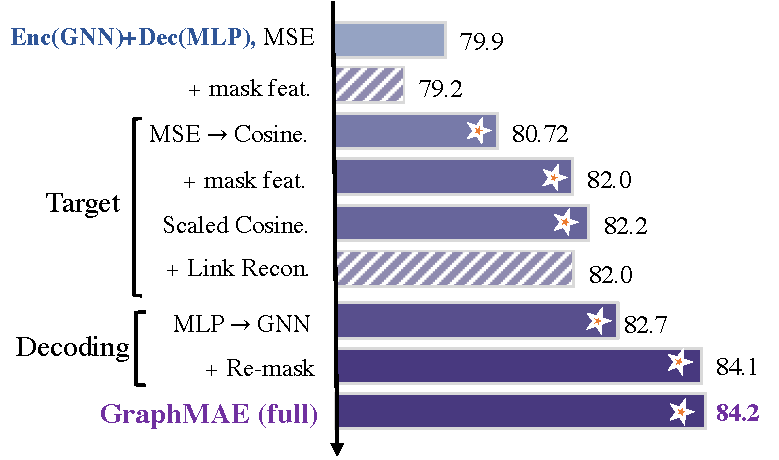
\includegraphics[width=0.48\textwidth]{imgs/GraphMAEXT.pdf}
%     \caption{ the effect of \model design. }
%     \label{fig:design_xt}
% \end{figure}


% -----------------



















\hide{ %%%%%==============================

\section{Introduction}%
\label{sec:introduction}
Self-supervised learning (SSL), which can be generally categorized into generative and contrastive methods~\cite{liu2021self}, has found widespread adoption in computer vision (CV), natural language processing (NLP), and graph learning communities. 
While contrastive SSL methods have experienced a sudden emergence in the past two years, 
generative SSL is gaining steadily increasing significance thanks to several successful practices, including well-established BERT~\cite{devlin2019bert}, GPT~\cite{radford2019language} in NLP and very recent MAE~\cite{he2021masked}, iBOT~\cite{zhou2021ibot} in CV.



Generative SSL in graph, including graph autoregressive (GAR) and graph autoencoders (GAEs), has also been studied for long. 
As a typical GAR model, GPT-GNN~\cite{hu2020gpt} proposes an autoregressive framework to perform node and edge reconstruction iteratively. 
For GAEs, VGAE~\cite{kipf2016variational} is a pioneer which targets predicting missing edges.
EP~\cite{garcia2017learning} first propose to recover vertex features. 
Later GAEs, including ARVGA~\cite{pan2018adversarially}, MGAE~\cite{wang2017mgae}, GALA~\cite{park2019symmetric}, GATE~\cite{amin2020gate}, and AGE~\cite{cui2020adaptive} majorly focus on challenges of link prediction and graph clustering. 
Compared to GAR's impractical assumption on graph generating orders, GAEs holds little assumption and thus find more widespread applications.

However, in the context of graph learning, albeit prior efforts on GAEs, 
contrastive SSL is still the dominant approach, especially for node and graph classification. 
Its success has been built upon complex designs and architectures. 
For example, bi-encoders with momentum update, exponential moving average (EMA), and Stop-Gradient are usually indispensable to stabilize the training (e.g., GCC~\cite{qiu2020gcc}, BGRL~\cite{thakoor2021bootstrapped}). 
Negative samples are necessary for most contrastive training objectives, but often require arduous labour to sample or construct from graphs (e.g., GRACE~\cite{zhu2020deep}, GCA~\cite{zhu2021graph}). 
Sometimes, further transformation are needed to create even harder negatives (e.g., DGI~\cite{velivckovic2018deep}). 
Finally, heavy reliance on high-quality and label-invariant data augmentation proves to be the Achilles heel of contrastive SSL (e.g., CCA-SSG~\cite{zhang2021canonical}). 
These augmentation techniques are mostly based on heuristics whose effectiveness vary drastically from graph to graph, and some of them can be unscalable at larger scales (e.g., diffusion in MVGRL~\cite{hassani2020contrastive}).

\vpara{Dilemma.} 
Self-supervised GAEs can naturally avoid aforementioned conflicts of contrastive methods, but suffer from poor performance on node and graph classification. 
Despite a number of recent attempts~\cite{you2020does,manessi2021graph,zhu2020self,jin2020self,hu2020strategies} to handle such challenges with autoencoders, none of them succeed in achieving a comprehensive outperform over state-of-the-art contrastive SSL methods; 
the progress of GAEs in graph has lagged behind NLP and CV. To bridge the gap, we systematically analysis the deficiency of existing GAEs:
%We try to shed some lights on this gap by analyzing the following problems of existing GAEs:

(i) Proximity information is over-emphasized. 
Most existing GAEs leverage the structure reconstruction as the main task to encourage topological closeness between neighbour nodes.
Consequently, prior GAEs are usually good at link prediction and clustering, but unsatisfactory on classification.

(ii) Feature reconstruction without corruption is not robust. 
For GAEs that introduce the task of feature reconstruction, 
most of them still employ the vanilla architecture that risks to learn trivial solutions, rather than the more efficient denoising autoencoders~\cite{vincent2008extracting} which corrupt input and then recover.

(iii) Mean Square Error (MSE) criterion can be sensitive and unstable. 
To the best of our knowledge, all the existing GAEs with feature reconstruction have adopted MSE as their criterion. 
However, MSE is known to suffer from varied feature vector norms and curse of dimensionality, and thus can cause the collapse of training. 
%\todo{polish the reason}

(iv) Decoder architectures are of little expressiveness. 
Most GAEs leverage simple MLP as their decoders following BERT. 
However, while in language the targets are one-hot vectors containing rich semantics, in graphs most of our targets are less informative feature vectors (except for some discrete attributes such as in chemical graphs). 
In this case, trivial decoder design may not be strong enough to bridge the gap between encoder representations and decoder targets.

Noted that while previous works on GAEs may have individually tackled one or two of the above defects, none of them jointly deals with the four challenges as a whole to consequently present a unified GAE solution to supersede contrastive ones over extensive benchmarks.


\vpara{Contributions.}
In light of the above observations, we endeavor to revival the idea of generative GAEs by optimizing its design and assimilating the advantages individually appear in prior GAEs. 
We propose \model, a masked graph autoencoder with decoding enhancement, and find that the following crucial designs of \model can lead to substantially boosted performance on node classification, graph classification, and transfer learning: 

\textbf{Masked Feature Reconstruction}: 
\model focuses on feature reconstruction with the more challenging masked prediction objective, 
whose effectiveness and superiority over vanilla architecture has been verified in CV and NLP for long. 

\textbf{Cosine Error}: 
\model employs Cosine Error, which is beneficial when feature vectors vary in their magnitudes (as is often the case for node attributes in graphs), rather than traditional MSE. 
On top of it, we introduce a scaling factor $\gamma\ge 1$ to conquer the problem of imbalance between easy and hard to reconstruct samples.

\textbf{Re-mask Decoding}: 
\model enhance the design of decoder using a more expressive single-layer GNN instead of traditional MLP. 
A novel Re-mask Decoding strategy which re-masks encoder's output embeddings of masked input nodes brings additional improvements.

Surprisingly, without using any complicated tricks including data augmentation, negative sampling, bi-encoders and other techniques to stabilize training, 
\model achieves competitive and even much better performance on a wide range of node classification and graph classification benchmarks compared to state-of-the-art contrastive SSL approaches. 
It also significantly pushes the boundary of graph autoencoders, showing that generative SSL can offer great potential to graph representation learning in the future.


\begin{table}
    \centering
    \caption{Technical comparison between generative SSL methods. \textmd{\textit{AE}: autoencoder methods. \textit{No Struct.}: no structure reconstruction objective. \textit{Mask Feat.}: use masking to corrupt input features. \textit{GNN Decoder}: use GNN as the decoder. \textit{Space} refers to run-time memory consumption. \textit{CE} denotes Cross-Entropy Error.}}
    \vspace{-2mm}
    \small
    \begin{tabular}{@{}lccccccc@{}}
\toprule[1.2pt]
Methods  & \makecell[c]{Feat.\\Loss}   & AE         & \makecell[c]{No\\Struc.}  & \makecell[c]{Mask\\Feat.} & \makecell[c]{GNN\\Decoder}    & \makecell[c]{Re-mask\\Dec.}   & Space              \\ \midrule
VGAE~\cite{kipf2016variational} & n/a      & \Checkmark & -          & -          & -             & -    & $\mathcal{O}(N^2)$ \\
% EP~\cite{garcia2017learning}       & MSE    & \Checkmark & \Checkmark & -          & -            & -    & $\mathcal{O}(N^2)$ \\
ARVGA~\cite{pan2018adversarially}    & n/a      & \Checkmark & -          & -          & -          & -    & $\mathcal{O}(N^2)$ \\
MGAE~\cite{wang2017mgae}     & MSE    & \Checkmark & -          & \Checkmark & -                    & -    & $\mathcal{O}(N)$ \\
GALA~\cite{park2019symmetric}     & MSE    & \Checkmark & \Checkmark & -          & \Checkmark      & -    & $\mathcal{O}(N)$  \\
GATE~\cite{amin2020gate}     & MSE    & \Checkmark & -          & -          & \Checkmark           & -    & $\mathcal{O}(N)$   \\
AttrMask~\cite{hu2020strategies} & CE     & \Checkmark & \Checkmark & \Checkmark & -                & -    & $\mathcal{O}(N)$   \\
GPT-GNN~\cite{hu2020gpt}  & MSE    & -          & -          & \Checkmark & -                       & -    & $\mathcal{O}(N)$   \\
AGE~\cite{cui2020adaptive}     & n/a      & \Checkmark & -          & -          & -                & -    & $\mathcal{O}(N^2)$  \\
NodeProp~\cite{jin2020self} & MSE    & \Checkmark & \Checkmark & \Checkmark & -                     & -    & $\mathcal{O}(N)$ \\
% RASSL~\cite{zhu2020self}    & MSE    & \Checkmark & -          & -          & -           & $\mathcal{O}(N^2)$   \\ 
\midrule
% \model   & Cosine & \Checkmark & \Checkmark & \Checkmark & \Checkmark  & $\mathcal{O}(N)$ \\ \bottomrule[1.2pt]
\model   & SCE & \Checkmark & \Checkmark & \Checkmark & \Checkmark  & \Checkmark & $\mathcal{O}(N)$ \\ \bottomrule[1.2pt]
\end{tabular}

    \label{tab:ae_compare}
\end{table}

\begin{figure}
    \centering
    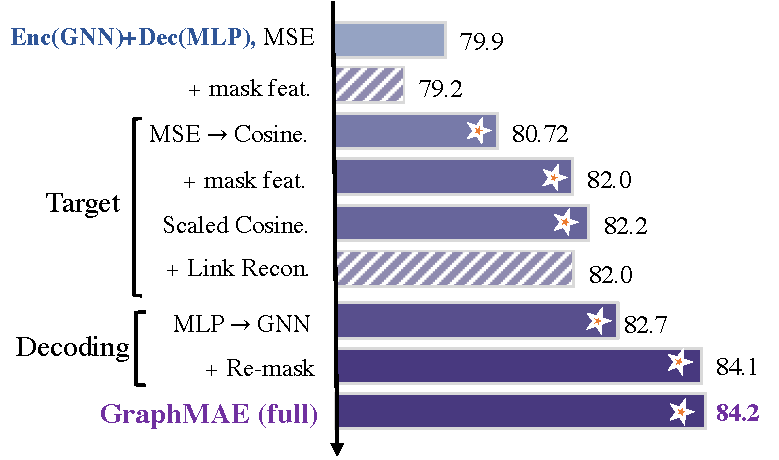
\includegraphics[width=0.48\textwidth]{imgs/GraphMAEXT.pdf}
    \caption{ the effect of \model design. }
    \label{fig:design_xt}
\end{figure}



}%========================================






\hide{
\begin{table}[t]
    \centering
    \caption{Technical comparison between \model and contrastive SSL methods. \textmd{Contrastive methods' performance relies on complicated bi-encoder architecture, negative sampling and strong data augmentation; \model do not need them at all.}}
    \vspace{-2mm}
    \small
    \renewcommand\tabcolsep{3pt}
    
\begin{tabular}{@{}clcccc@{}}
\toprule[1.2pt]
SSL                           & Methods & Bi-encoder & NegSample & DataAug    & Space \\ \midrule
\multirow{4}{*}{Contrastive} & MVGRL~\cite{hassani2020contrastive}   & \Checkmark & \Checkmark & \Checkmark & $\mathcal{O}(N^2)$      \\
                              & GCC~\cite{qiu2020gcc}     & \Checkmark & \Checkmark & \Checkmark & $\mathcal{O}(N)$        \\
                              & GraphCL~\cite{you2020graph} & -          & \Checkmark & \Checkmark & $\mathcal{O}(N^2)$      \\
                              & BGRL~\cite{thakoor2021bootstrapped}    & \Checkmark & -          & \Checkmark & $\mathcal{O}(N)$    \\ \midrule
Generative                    & \model                      & -          & -          & -          & $\mathcal{O}(N)$    \\ \bottomrule[1.2pt]
\end{tabular}
    \label{tab:contrastive_compare}
    \vspace{-5mm}
\end{table}
}


\hide{
%\clearpage
The idea of masked autoencoders, a form of more general denoising autoencoders, is natural and applicable in computer vision as well. Indeed, closely related research in vision preceded BERT. However, despite signif- icant interest in this idea following the success of BERT, progress of autoencoding methods in vision lags behind NLP. We ask: what makes masked autoencoding different between graph and vision? We attempt to answer this question.


Inspired by the success of contrastive learning in vision, similar methods have been adapted to learning graph neural networks. Although these models have achieved impressive performance, they require complex designs and architectures. For example, DGI and MVGRL rely on a parameterized mutual information estimator to discriminate positive node-graph pairs from negative ones; GRACE and GCA harness an additional MLP-projector to guarantee sufficient capacity. Moreover, negative pairs sampled or constructed from data often play an indispensable role in providing effective contrastive signals and have a large impact on performance. Selecting proper negative samples is often nontrivial for graph-structured data, not to mention the extra storage cost for prohibitively large graphs. BGRL is a recent endeavor on targeting a negative-sample-free approach for GNN learning through asymmetric architectures. However, it requires additional components, e.g., an exponential moving average (EMA) and Stop- Gradient, to empirically avoid degenerated solutions, leading to a more intricate architecture.
}